\section{Results}

\subsection{Cohort Audit and Why Split Regime Matters}
Auditing all 368,132 STS ACSD v2.81 isolated-CABG records across 1,091 U.S.\ centers recovered 367,695 labeled procedures (89,337 POAF events, 24.30\%; Table~\ref{tab:cohort}) and strictly 207 pre-incision predictors after removing seven early-column postoperative duration leaks and all intraoperative/postoperative fields. Across 928 U.S.\ centers performing $\ge 100$ procedures, hospital POAF incidence spanned a threefold range from 12.2\% to 34.2\% (5th--95th percentile; median 24.1\%; Fig.~\ref{fig:audit_splits}A).

A naive calendar-2017 holdout (61,552 cases across 983 centers) placed 99.5\% of test hospitals inside the 2014--2016 training set and exhibited +6.0 percentage points of missingness drift ($\mathrm{Max}\,|\mathrm{SMD}|=0.360$; Fig.~\ref{fig:audit_splits}B). An identical 207-feature CatBoost model scored 0.6778 on that overlapping 2017 split but dropped by $-1.99$ AUC points to 0.6579 on 2017 patients treated at strictly unseen hospitals ($n{=}3{,}555$, 63 centers). Separating external cold-start evaluation (Regime 1: 74 strictly unseen centers, 0.0\% overlap, $\mathrm{Max}\,|\mathrm{SMD}|=0.103$) from controlled in-network evaluation (Regime 2: all 1,091 centers represented in training, 100.0\% overlap) eliminated this confounding cleanly.

\begin{table*}[t]
\centering
\caption{\ct{National STS ACSD v2.81 Isolated-CABG Cohort and Two Controlled Validation Regimes ($N{=}367{,}695$ Labeled Procedures Across 1,091 U.S.\ Surgical Centers).}}
\label{tab:cohort}
\tablefont
\setlength{\tabcolsep}{4.2pt}
\begin{tabularx}{\textwidth}{@{}Y R{2.05cm} R{2.35cm} R{2.35cm} R{2.35cm}@{}}
\toprule
\thd{Cohort Characteristic / Split Design} & \thd{Full Cohort} & \thd{Regime 1: Unseen Train / Test} & \thd{Regime 2: Seen Train / Test} & \thd{Calendar-2017 (Naive)} \\
\midrule
Procedures, $n$ (POAF Events, \%) & 367,695 (24.30\%) & 50,000 / 21,241 (24.29\%) & 50,000 / 21,241 (24.30\%) & 306,143 / 61,552 (24.83\%) \\
Surgical Centers in Train / Test & 1,091 total & 1,017 / 74 & 1,091 / 1,086 & 1,090 / 983 \\
Test Hospital Overlap With Train (\%) & --- & \textbf{0.0\%} (74 unseen) & \textbf{100.0\%} (0 unseen) & 99.5\% (63 unseen) \\
Strictly Pre-Incision Predictors & 207 raw & 207 raw & 207 raw / 208 site & 207 raw \\
Age, mean $\pm$ SD (yr) & 65.1 $\pm$ 10.1 & 65.2 $\pm$ 10.1 (test) & 65.1 $\pm$ 10.1 (test) & 65.7 $\pm$ 9.7 \\
Female Sex, \% & 25.2\% & 24.4\% & 24.4\% & 23.7\% \\
Diabetes / Heart Failure / Urgent, \% & 48.6\% / 21.7\% / 58.4\% & 49.2\% / 23.6\% / 58.6\% & 48.0\% / 19.0\% / 52.6\% & 48.9\% / 19.4\% / 53.5\% \\
Hospital POAF Rate Dispersion (5th--95th) & 12.2\%--34.2\% & Matched (Max|SMD| 0.103) & Stratified across all sites & Missingness drift +6.0 pp \\
\bottomrule
\end{tabularx}
\vspace{2pt}
{\raggedright\sffamily\fontsize{6.9}{8.6}\selectfont\color{sub}All 50,000-patient parity cohorts are exact 50:50 class-balanced across five hospital-grouped CV folds; every model is evaluated at natural clinical prevalence ($\approx$24.3\%) using unified fold-OOF Platt calibration plus development-only Bayes prior shift ($-1.1365$).\par}
\end{table*}


\begin{figure*}[t]
  \centering
  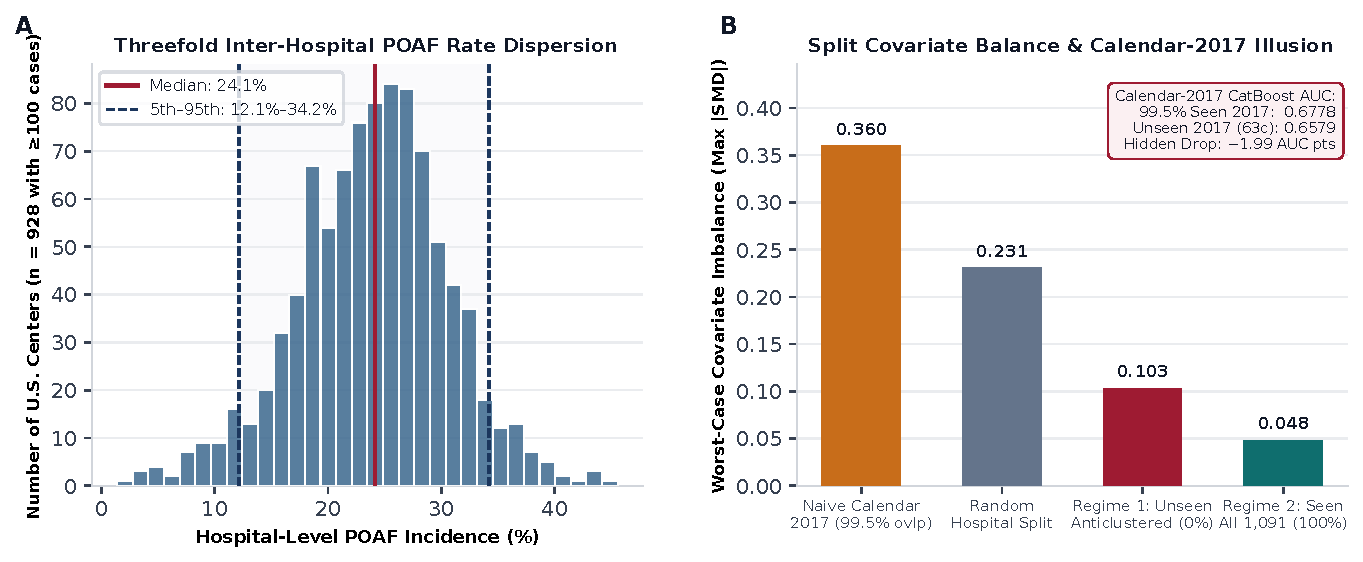
\includegraphics[width=0.96\textwidth]{figures/fig2_cohort_audit_and_split_regimes.pdf}
  \caption{\ct{Inter-Hospital POAF Rate Dispersion and Split-Geometry Leakage Audit.} \textbf{A},~Threefold dispersion in hospital-level POAF incidence across 928 U.S.\ surgical centers with $\ge 100$ procedures (median 24.1\%; 5th--95th percentile 12.2\%--34.2\%). \textbf{B},~Worst-case covariate imbalance ($\mathrm{Max}\,|\mathrm{SMD}|$) across split designs; callout highlights the $-1.99$ AUC-point decline of a matched 207-predictor CatBoost model between overlapping calendar-2017 evaluation (0.6778) and strictly unseen 2017 hospitals (0.6579).}
  \label{fig:audit_splits}
\end{figure*}

\subsection{Regime 1: Unseen-Hospital Cold Start (0\% Overlap)}
Across 74 strictly unseen holdout hospitals ($N{=}21{,}241$, 5,160 events; Table~\ref{tab:benchmark} and Fig.~\ref{fig:hero}A), \textbf{NEVERHUMAN} achieved the highest 50,000-patient ROC-AUC at \textbf{0.6767} (95\% CI 0.6686--0.6858), highest average precision (\textbf{0.3777}), and sharp calibration (ECE \textbf{0.0072}, slope 0.983, O:E 0.994). NEVERHUMAN outperformed every single binary alternative with 5,000-draw 74-hospital cluster 95\% CIs strictly excluding zero:
\begin{itemize}
  \item \textbf{+21.8\,bps} $[+7.0, +36.5]$ ($P{>}0 = 0.998$) vs.\ \textbf{AutoGluon 1.5} (\cli{best\_quality}, 0.6745);
  \item \textbf{+24.5\,bps} $[+7.2, +42.2]$ ($P{>}0 = 0.997$) vs.\ \textbf{CatBoost} (5-fold binary, 0.6742);
  \item \textbf{+29.2\,bps} $[+8.2, +53.5]$ ($P{>}0 = 0.998$) vs.\ \textbf{PriorLabs TabPFN-3.5} (0.6738);
  \item \textbf{+52.0\,bps} $[+21.6, +83.3]$ ($P{>}0 = 1.000$) vs.\ \textbf{NVIDIA KumoTabular-Large v2} (0.6715);
  \item \textbf{+55.3\,bps} $[+28.6, +81.5]$ ($P{>}0 = 1.000$) vs.\ \textbf{Google TabFM v1.0.0} (0.6712); and
  \item \textbf{+577.0\,bps} $[+495.6, +656.9]$ ($P{>}0 = 1.000$) vs.\ the reconstructed \textbf{Mariscalco POAF} bedside score (0.6190).
\end{itemize}
Trained on 50,000 cases, NEVERHUMAN closed \textbf{79.2\%} of the discrimination gap to a $7\times$ larger 346,454-patient CatBoost model (0.6773; difference $-6.4$\,bps $[-23.0, +10.5]$, non-significant) while outperforming that $7\times$ full-registry model on both average precision (0.3777 vs.\ 0.3776) and calibration error (ECE 0.0072 vs.\ 0.0076).

\begin{table*}[t]
\centering
\caption{\ct{Head-to-Head Pre-Incision POAF Discrimination Across Both Regimes: Unseen Hospitals (74 Centers, 0\% Overlap) and Seen Hospitals (1,086 Centers, 100\% Overlap; $N{=}21{,}241$ Natural-Prior Holdouts).}}
\label{tab:benchmark}
\tablefont
\setlength{\tabcolsep}{3.2pt}
\begin{tabularx}{\textwidth}{@{}Y R{2.55cm} R{2.75cm} R{0.95cm} R{0.95cm} R{1.15cm} R{1.15cm} R{1.20cm}@{}}
\toprule
\thd{Model (50k Binary Parity Unless Noted)} & \thd{Unseen AUC (95\% CI)} & \thd{NEVERHUMAN $\Delta$ Unseen (bps)} & \thd{Unseen AP} & \thd{Unseen ECE} & \thd{Seen 207 Raw} & \thd{Seen Native 208} & \thd{Seen +EB346k} \\
\midrule
\multicolumn{8}{@{}l@{}}{\sffamily\bfseries\fontsize{6.7}{8.1}\selectfont\color{navy}Tier 1: Proprietary Champion vs.\ Five Binary Tabular AI Alternatives (Identical 50,000-Patient Cohort, 207 Pre-Incision Features)} \\
\rowcolor{primarytint}
\textbf{NEVERHUMAN (Proprietary)} & \textbf{0.6767 (0.669--0.686)} & \textbf{Reference (\#1 @ 50k)} & \textbf{0.3777} & \textbf{0.0072} & \textbf{0.6794} & \textbf{0.6916} & \textbf{0.6974} \\
AutoGluon 1.5 (best\_quality) & 0.6745 (0.666--0.684) & +21.8 [+7.0, +36.5]$^\ast$ & 0.3743 & 0.0046 & 0.6790 & 0.6891 & 0.6974 \\
CatBoost (5-Fold Binary) & 0.6742 (0.666--0.683) & +24.5 [+7.2, +42.2]$^\ast$ & 0.3744 & 0.0078 & 0.6777 & 0.6886 & 0.6966 \\
PriorLabs TabPFN-3.5 (50k Native) & 0.6738 (0.666--0.683) & +29.2 [+8.2, +53.5]$^\ast$ & 0.3728 & 0.0068 & 0.6795 & --- & 0.6982 \\
NVIDIA KumoTabular-Large v2 & 0.6715 (0.663--0.681) & +52.0 [+21.6, +83.3]$^\ast$ & 0.3693 & 0.0070 & 0.6764 & --- & 0.6977 \\
Google TabFM v1.0.0 & 0.6712 (0.663--0.680) & +55.3 [+28.6, +81.5]$^\ast$ & 0.3697 & 0.0090 & 0.6775 & --- & 0.6986 \\
\midrule
\multicolumn{8}{@{}l@{}}{\sffamily\bfseries\fontsize{6.7}{8.1}\selectfont\color{navy}Tier 2: Clinical Bedside Proxy \& 7$\times$ Full-Registry Scaling Reference} \\
Mariscalco POAF Bedside Proxy & 0.6190 (0.610--0.628) & +577.0 [+495.6, +656.9]$^\ast$ & 0.3097 & 0.0190 & 0.6276 & --- & --- \\
CatBoost Full Registry (346k, 7$\times$) & 0.6773 (0.670--0.686) & $-$6.4 [$-$23.0, +10.5] & 0.3776 & 0.0076 & 0.6831 & \textbf{0.7014} & --- \\
\bottomrule
\end{tabularx}
\vspace{2pt}
{\raggedright\sffamily\fontsize{6.8}{8.5}\selectfont\color{sub}All 95\% CIs use 5,000 whole-hospital cluster bootstrap draws (seed 42; 74 unseen hospitals / 1,086 seen hospitals). $^\ast$95\% cluster CI strictly excludes zero. Native 50k site-aware (\cli{site208}) NEVERHUMAN reaches 0.6916, leading CatBoost \cli{site208} (0.6886) by +29.0\,bps [+16.6, +41.5]${}^\ast$ and AutoGluon \cli{site208} (0.6891) by +24.1\,bps [+12.5, +35.4]${}^\ast$. Closed-form train-only Empirical-Bayes hospital priors (+EB346k) lift every 50k model into 0.696--0.699 and 346k CatBoost to 0.7014.\par}
\end{table*}


\subsection{Regime 2: Seen-Hospital In-Network Performance (100\% Overlap)}
Evaluating the exact same six models on the matched 100\% Seen-Hospital split (all 1,091 U.S.\ centers present in training; $N{=}21{,}241$ across 1,086 seen centers; Table~\ref{tab:benchmark} and Fig.~\ref{fig:seen_unseen}) yielded two central insights.

First, even with \emph{zero} hospital identifier input (207 patient variables only), seeing test hospitals during training inflated every model's ROC-AUC by \textbf{+28 to +64\,bps} relative to unseen hospitals. Tabular foundation models experienced roughly twice the familiarity boost (+49 to +64\,bps) observed for NEVERHUMAN (+28\,bps). On seen patient-only features, NEVERHUMAN (0.6794) strictly outperformed Kumo (+30.4\,bps $[+12.8, +48.1]$), TabFM (+18.9\,bps $[+2.8, +35.3]$), and CatBoost (+16.9\,bps $[+5.1, +28.7]$), edged AutoGluon (0.6790; +4.1\,bps), and matched TabPFN-3.5 (0.6795; $-0.4$\,bps) while scoring patients 125$\times$ faster.

Second, incorporating each center's strictly train-only Empirical-Bayes hospital POAF prior lifted every model into the 0.69--0.70 clinical frontier (Fig.~\ref{fig:seen_unseen}A--B). Under native end-to-end 50k site-aware training (\cli{site208}), \textbf{NEVERHUMAN led at 0.6916} (95\% CI 0.6844--0.6987), beating both \textbf{AutoGluon \cli{site208}} (0.6891) by \textbf{+24.1\,bps} $[+12.5, +35.4]$ ($P{>}0 = 1.000$) and \textbf{CatBoost \cli{site208}} (0.6886) by \textbf{+29.0\,bps} $[+16.6, +41.5]$ ($P{>}0 = 1.000$). Closed-form updating with full-registry historical site priors (+$\mathrm{EB}_{346\mathrm{k}}$) lifted all 50k models by +179 to +213\,bps into a tight 0.6966--0.6986 band (NEVERHUMAN 0.6974, AutoGluon 0.6974, CatBoost 0.6966, TFMs 0.6977--0.6986; all pairwise cluster CIs spanning zero), while $7\times$ 346k site-aware CatBoost defined the upper registry ceiling at \textbf{0.7014} (slope 1.014, O:E 0.999).

\begin{figure*}[t]
  \centering
  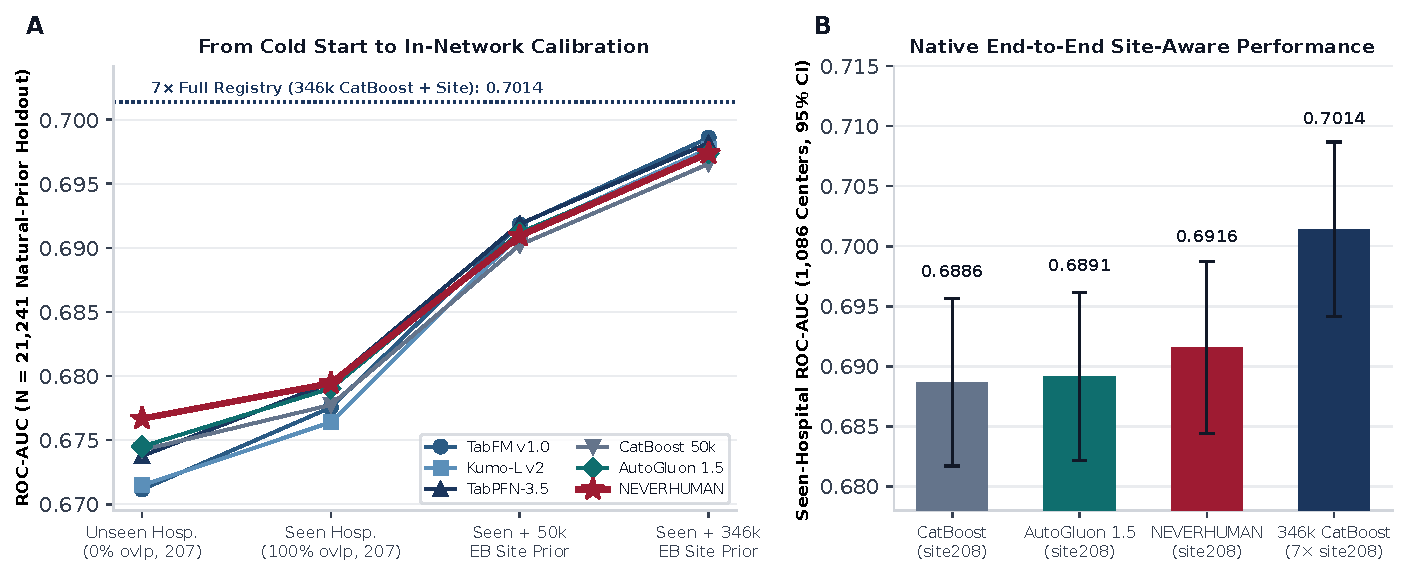
\includegraphics[width=0.96\textwidth]{figures/fig3_unseen_vs_seen_hospitals.pdf}
  \caption{\ct{Cold-Start Unseen Hospitals vs.\ In-Network Seen Hospitals and Site Calibration.} \textbf{A},~Paired ROC-AUC progression across all six models from strictly unseen hospitals (0\% overlap) to seen hospitals (207 patient features only) and train-only Empirical-Bayes hospital priors (+$\mathrm{EB}_{50\mathrm{k}}$, +$\mathrm{EB}_{346\mathrm{k}}$). \textbf{B},~Native end-to-end site-aware (\cli{site208}) ROC-AUC with 1,086-hospital cluster 95\% CIs, where NEVERHUMAN (0.6916) leads both AutoGluon (0.6891) and CatBoost (0.6886).}
  \label{fig:seen_unseen}
\end{figure*}

\subsection{Training and Inference Speed Showcase}
Clinical deployment requires real-time bedside scoring without prohibitive multi-GPU serving clusters. Table~\ref{tab:timing} and Fig.~\ref{fig:timing} report exact wall-clock training/preparation times, full-cohort inference times across all 21,241 holdout patients, per-patient latencies, and peak GPU VRAM across all six models.

\begin{itemize}
  \item \textbf{Tabular Foundation Models (In-Context Bottleneck):} Although TabPFN-3.5 requires minimal context preparation (0.9\,s), all three TFMs must attend over 10,000--50,000 training rows during inference. Scoring 21,241 patients on an NVIDIA A100-40GB GPU required \textbf{481.7\,s} (22.7\,ms/patient; 6.8\,GB allocated / 12.0\,GB reserved VRAM) for KumoTabular-Large v2, \textbf{515.3\,s} (24.3\,ms/patient; 7.7\,GB / 14.7\,GB VRAM) for TabPFN-3.5, and \textbf{1,326.7\,s} (62.5\,ms/patient; 22.1\,GB / 40.8\,GB VRAM) for TabFM v1.0.0.
  \item \textbf{AutoGluon 1.5 (\cli{best\_quality}):} Exhausted the full \textbf{30.0-minute} (1,797.1\,s) training budget, accumulated \textbf{10.1\,GB} of serialized ensemble artifacts (9.9--11.2\,GB across splits), and required \textbf{80.99\,s} for 21,241-patient unseen batch scoring (3.81\,ms/patient; 4.80\,s on seen raw207 and 37.78\,s on \cli{site208}) and \textbf{28.5\,s} for single-patient bedside scoring when bagged random forests entered the final weighted ensemble.
  \item \textbf{CatBoost (5-Fold Binary):} Fastest overall (49.2\,s training on 20 CPU threads; 0.15\,s batch inference, 0.007\,ms/patient, 3.0\,ms single-patient), but trailed NEVERHUMAN by $-24.5$\,bps on unseen hospitals and $-29.0$\,bps on native \cli{site208} seen hospitals.
  \item \textbf{NEVERHUMAN (Pareto-Optimal Champion):} Completed offline training in \textbf{21.5\,minutes} (1,290.7\,s---28\% faster than AutoGluon) and scored all 21,241 patients in \textbf{4.11\,s} (\textbf{0.193\,ms/patient}; \textbf{45.2\,ms} single-patient bedside latency; \textbf{0.53\,GB} peak GPU VRAM)---\textbf{19.7$\times$ faster} than AutoGluon on unseen batch inference (\textbf{630$\times$ faster} single-patient), \textbf{117$\times$ faster} than Kumo, \textbf{125$\times$ faster} than TabPFN-3.5, and \textbf{323$\times$ faster} than TabFM while using \textbf{13$\times$--42$\times$ less GPU VRAM} and delivering the highest accuracy (Fig.~\ref{fig:timing}C).
\end{itemize}

\begin{table*}[t]
\centering
\caption{\ct{Training Wall-Clock Time, Batch Inference Speed ($N{=}21{,}241$ Holdout Patients), Single-Patient Latency, and Compute Footprint Across All Six Evaluated Models.}}
\label{tab:timing}
\tablefont
\setlength{\tabcolsep}{3.2pt}
\begin{tabularx}{\textwidth}{@{}Y R{1.05cm} R{1.75cm} R{1.35cm} R{1.25cm} R{1.30cm} R{1.65cm} L{2.55cm}@{}}
\toprule
\thd{Model (50k Train $\to$ 21,241 Test)} & \thd{Unseen AUC} & \thd{Train / Prep Time} & \thd{21k Batch Infer} & \thd{Batch ms/pt} & \thd{1-Pt Latency} & \thd{Infer Speed vs.\ NH} & \thd{Hardware (Peak VRAM)} \\
\midrule
\rowcolor{primarytint}
\textbf{NEVERHUMAN} & \textbf{0.6767} & \textbf{1290.7\,s (21.5\,m)} & \textbf{4.11\,s} & \textbf{0.193} & \textbf{45.2\,ms} & \textbf{1.0$\times$ (Ref)} & 1x RTX 3090 + CPU (0.5\,GB VRAM) \\
CatBoost (5-fold binary) & 0.6742 & 49.20\,s & 0.15\,s & 0.007 & 3.0\,ms & 28.0$\times$ faster & CPU (20 threads) (CPU) \\
AutoGluon 1.5 (best\_quality) & 0.6745 & 1797.1\,s (30.0\,m) & 80.99\,s & 3.81 & 28.5\,s & 19.7$\times$ slower & 1x RTX 4090 + 48 CPUs (10.1\,GB disk) \\
NVIDIA KumoTabular-Large v2 & 0.6715 & 197.1\,s (3.3\,m) & 481.69\,s & 22.68 & In-context & 117.3$\times$ slower & A100 40GB (6.8\,GB VRAM) \\
PriorLabs TabPFN-3.5 & 0.6738 & 0.89\,s & 515.29\,s & 24.26 & In-context & 125.4$\times$ slower & A100 40GB (7.7\,GB VRAM) \\
Google TabFM v1.0.0 & 0.6712 & 394.9\,s (6.6\,m) & 1326.73\,s & 62.46 & In-context & 323.0$\times$ slower & A100 40GB (22.1\,GB VRAM) \\
\bottomrule
\end{tabularx}
\vspace{2pt}
{\raggedright\sffamily\fontsize{6.8}{8.5}\selectfont\color{sub}Batch inference measures wall-clock time to score all 21,241 unseen-hospital patients (median of 3 passes for NEVERHUMAN, CatBoost, and AutoGluon; verified offline GPU receipts for TabPFN-3.5, KumoTabular-Large v2, and TabFM v1.0.0). Tabular foundation models require passing the full 10k--50k training context through multi-layer attention at inference time, making batch scoring 117$\times$--323$\times$ slower than NEVERHUMAN while requiring 7--41\,GB GPU VRAM.\par}
\end{table*}


\begin{figure*}[t]
  \centering
  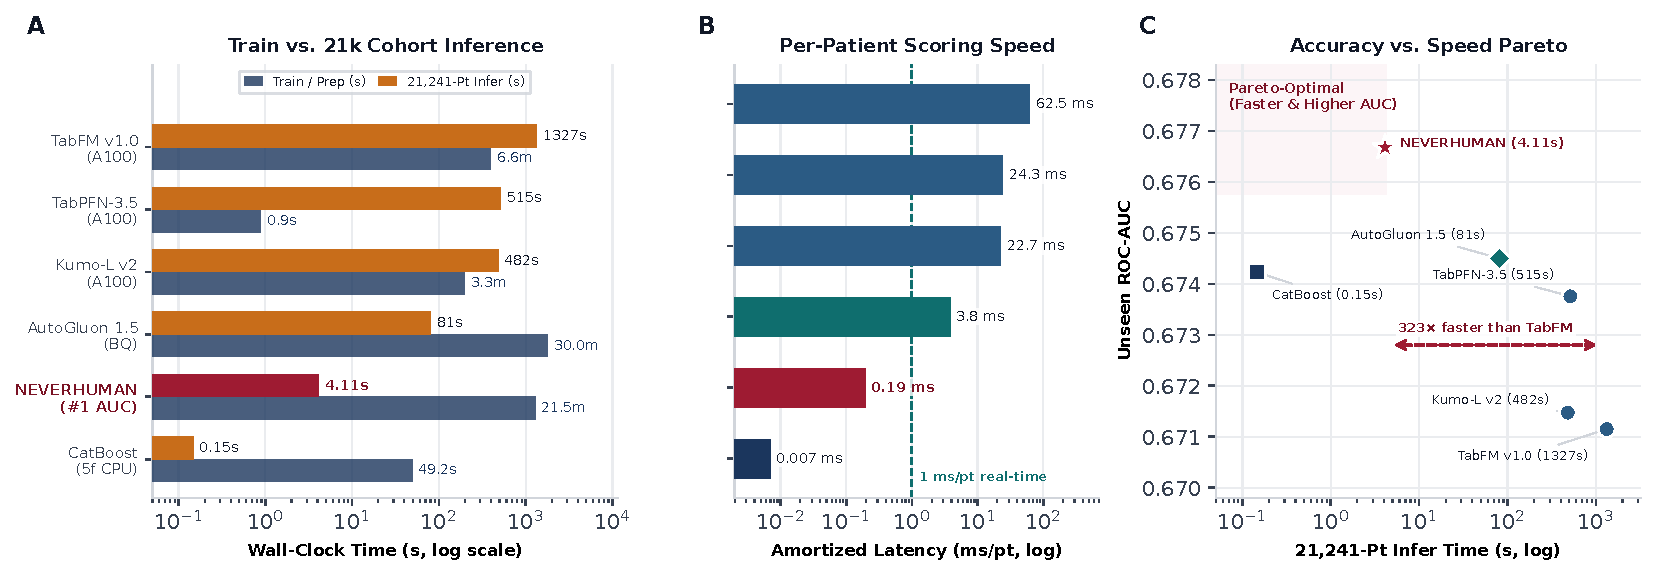
\includegraphics[width=0.98\textwidth]{figures/fig4_train_and_inference_efficiency.pdf}
  \caption{\ct{Training Time, Inference Speed ($N{=}21{,}241$), and Accuracy-vs-Speed Pareto Frontier.} \textbf{A},~Offline training/preparation time versus 21,241-patient batch inference time (log scale). \textbf{B},~Amortized per-patient scoring latency ($\mathrm{ms/patient}$, log scale), showing NEVERHUMAN (0.19\,ms/patient) and CatBoost cleanly below the 1\,ms real-time threshold. \textbf{C},~Accuracy versus inference-speed Pareto frontier illustrating NEVERHUMAN alone in the faster, more accurate top-left optimum.}
  \label{fig:timing}
\end{figure*}

\subsection{False-Positive Reduction and U.S./Global Surgical Impact}
Across all 367,695 labeled STS isolated-CABG procedures, patients who developed POAF experienced nearly double the unadjusted operative mortality (\textbf{2.78\% vs.\ 1.42\%}, excess +1.36 percentage points, 1.96$\times$), double the rate of prolonged ventilation (11.03\% vs.\ 5.52\%, 2.00$\times$), triple the rate of renal failure (3.48\% vs.\ 1.14\%, 3.05$\times$), and double the rate of cardiac arrest (2.36\% vs.\ 1.15\%, 2.05$\times$).

On the 74 strictly unseen hospitals, NEVERHUMAN stratified POAF risk monotonically across a \textbf{7.4-fold} decile gradient (6.07\% $\to$ 44.82\%; slope 0.983, O:E 0.994, ECE 0.0072; Fig.~\ref{fig:clinical}A), avoided \textbf{20.4--33.8 unnecessary prophylactic interventions per 100 patients} in Decision Curve Analysis (25\%--35\% thresholds; $P{>}0 = 1.000$ vs.\ Mariscalco POAF; Fig.~\ref{fig:clinical}B; Supplementary Table~S1), outperformed CatBoost 50k in \textbf{24 of 25 prespecified subgroups} (Supplementary Table~S2), and cut chronological 2014--2016 $\to$ 2017 center-level MAE by \textbf{14\%} (5.63 $\to$ 4.84\,pp).

Directly comparing False Positive Rates (FPR) at fixed clinical sensitivity targets demonstrates how risk-sorting accuracy scales across national (\textbf{200,000 U.S.\ isolated CABGs/year}) and global (\textbf{1,000,000 adult cardiac surgeries/year}\cite{vervoort2023global}) volumes (Table~\ref{tab:fpr_impact} and Fig.~\ref{fig:clinical}C):
\begin{itemize}
  \item \textbf{Lowest False Positive Rate at 70\% and 80\% POAF Capture:} To capture 70\% of POAF cases before incision on unseen hospitals, NEVERHUMAN incurred the lowest FPR of any model (\textbf{44.10\%} vs.\ 44.42\% AutoGluon, 44.58\% CatBoost, 44.76\% TabPFN-3.5, 45.14\% TabFM, 45.28\% Kumo, and 76.30\% Mariscalco POAF)---and dropped further to \textbf{41.22\%} on seen \cli{site208} hospitals. Scaled annually, NEVERHUMAN spares \textbf{490 to 1,798 U.S.\ patients/year} (\textbf{2,448 to 8,992 globally}) from needless prophylactic exposure versus the five binary AI alternatives, and \textbf{48,755 U.S.\ patients/year} (\textbf{243,774 globally}) versus Mariscalco POAF. At 80\% capture, NEVERHUMAN again achieved the lowest FPR (\textbf{55.54\%}), sparing 424--2,184 U.S.\ patients/year (2,118--10,921 globally) versus AI comparators.
  \item \textbf{Top-25\% Risk Sorting and Modeled Clinical Burden Averted:} Under a targeted Top-25\% pre-incision prophylaxis program (e.g., posterior left pericardiotomy, PALACS RCT 45\% relative risk reduction;\cite{gaudino2021palacs} sensitivity range 35\%--45\%), NEVERHUMAN captures \textbf{19,462 true POAF patients/year in the U.S.}\ (38.93\% PPV; +56 to +179 more cases/year than the five AI models and +2,552 more than Mariscalco POAF) and \textbf{97,312/year globally}. Modeled at 45\% efficacy, targeted NEVERHUMAN prophylaxis prevents \textbf{8,758 POAF episodes/year in the U.S.}\ (6,812--8,758 sensitivity range; \textbf{43,790/year globally})---yielding an estimated \textbf{\$87.6M--\$131.4M/year} in U.S.\ hospital cost avoidance.\cite{lapar2014poaf} Applying conservative 25\%--50\% causal attribution to our empirical +1.36\,pp STS operative mortality excess (100\% upper bound), this corresponds to \textbf{30--60 (upper 119) modeled U.S.\ operative deaths averted/year} (\textbf{149--298, upper 596 globally}) versus untargeted care, and \textbf{+4--8 (upper 16) additional U.S.\ lives/year} (\textbf{+20--39, upper 78 globally}) over bedside Mariscalco sorting.
\end{itemize}

\begin{table*}[t]
\centering
\caption{\ct{False Positive Rate (FPR) Comparison and Population-Scaled Clinical Impact Across 200,000 Annual U.S.\ CABG Procedures and 1,000,000 Global Cardiac Surgeries (74 Unseen Hospitals, $N{=}21{,}241$).}}
\label{tab:fpr_impact}
\tablefont
\setlength{\tabcolsep}{2.9pt}
\begin{tabularx}{\textwidth}{@{}Y R{1.25cm} R{1.25cm} R{1.60cm} R{1.65cm} R{1.20cm} R{1.60cm} R{2.20cm}@{}}
\toprule
\thd{Model (50k Parity)} & \thd{FPR @ 70\% Sens} & \thd{FPR @ 80\% Sens} & \thd{FP Spared / yr (200k U.S.)} & \thd{FP Spared / yr (1M Global)} & \thd{Top-25\% PPV} & \thd{NH Extra POAF (U.S. / yr)} & \thd{Modeled Prevented (U.S. / Global)} \\
\midrule
\rowcolor{primarytint}
\textbf{NEVERHUMAN (Proprietary)} & \textbf{44.10\%} & \textbf{55.54\%} & \textbf{Ref (Lowest)} & \textbf{Ref (Lowest)} & \textbf{38.93\%} & \textbf{Ref (Highest)} & \textbf{8,758 / 43,790} \\
AutoGluon 1.5 (best\_quality) & 44.42\% & 55.97\% & +490 & +2,448 & 38.68\% & +122 & 8,703 / 43,515 \\
CatBoost (5-Fold Binary) & 44.58\% & 55.86\% & +734 & +3,672 & 38.74\% & +94 & 8,716 / 43,578 \\
PriorLabs TabPFN-3.5 & 44.76\% & 55.82\% & +1,007 & +5,037 & 38.81\% & +56 & 8,733 / 43,663 \\
Google TabFM v1.0.0 & 45.14\% & 56.98\% & +1,582 & +7,909 & 38.81\% & +56 & 8,733 / 43,663 \\
NVIDIA KumoTabular-Large v2 & 45.28\% & 56.24\% & +1,798 & +8,992 & 38.57\% & +179 & 8,678 / 43,388 \\
Mariscalco POAF Bedside Proxy & 76.30\% & 76.30\% & +48,755 & +243,774 & 33.82\% & +2,552 & 7,610 / 38,049 \\
\bottomrule
\end{tabularx}
\vspace{2pt}
{\raggedright\sffamily\fontsize{6.75}{8.4}\selectfont\color{sub}Empirical FPRs and Top-25\% risk-sorting positive predictive values (PPV) are measured directly on the 74-unseen-hospital holdout ($N{=}21{,}241$; 24.29\% POAF) and scaled linearly to 200,000 annual U.S.\ isolated-CABG procedures (STS ACSD/AHA) and 1,000,000 annual global adult cardiac surgeries.\cite{vervoort2023global} Modeled POAF episodes prevented assume PALACS randomized trial efficacy for targeted posterior left pericardiotomy (45\% relative risk reduction; 35\%--45\% sensitivity range: 6,812--8,758 U.S.\ / 34,059--43,790 global).\cite{gaudino2021palacs} Across all 367,695 STS cases, POAF carried a +1.36-percentage-point unadjusted operative mortality excess (2.78\% vs.\ 1.42\%, 1.96$\times$); under conservative 25\%--50\% causal mortality attribution (100\% upper bound), Top-25\% NEVERHUMAN prophylaxis corresponds to 30--60 (upper 119) modeled U.S.\ operative deaths averted/yr (149--298, upper 596 globally) and \$87.6M--\$131.4M/yr in U.S.\ hospital costs.\cite{lapar2014poaf}\par}
\end{table*}


\begin{figure*}[t]
  \centering
  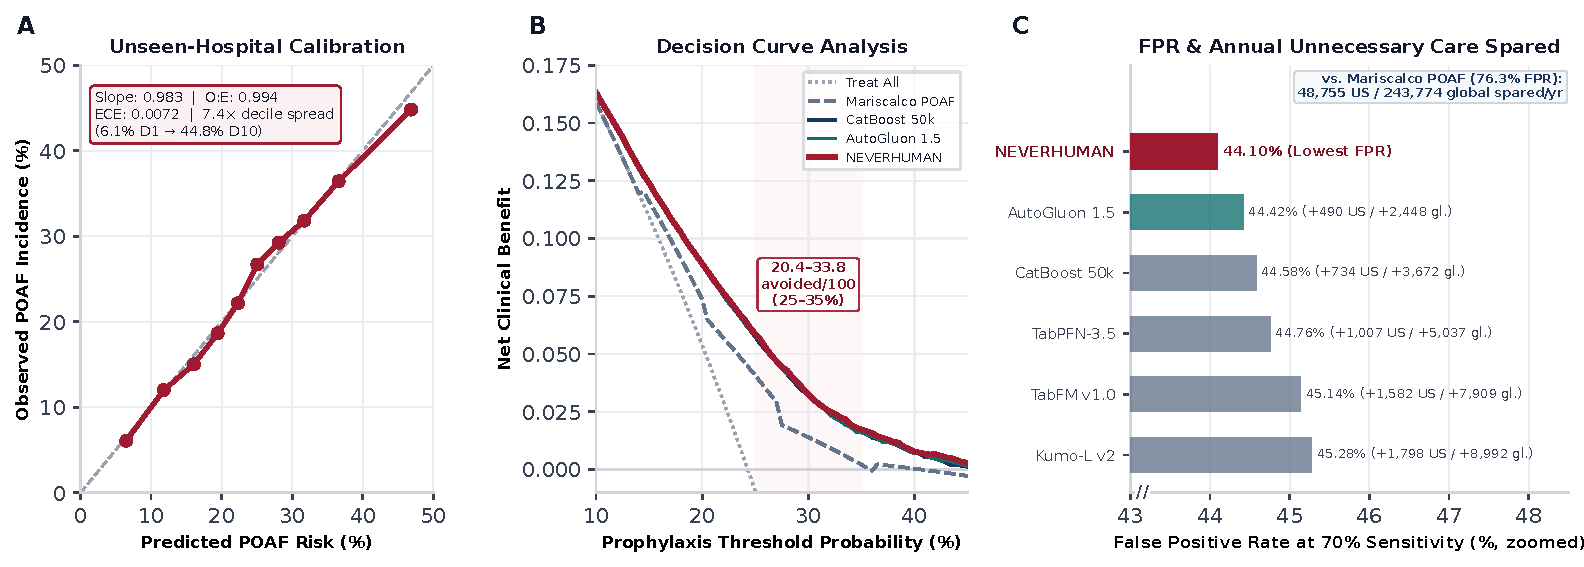
\includegraphics[width=0.98\textwidth]{figures/fig5_clinical_utility_calibration_equity.pdf}
  \caption{\ct{Unseen-Hospital Calibration, Decision Curve Clinical Utility, and False-Positive Reduction Scaled to U.S.\ and Global Cardiac Surgery Volumes.} \textbf{A},~Decile reliability curve demonstrating 7.4-fold monotonic POAF stratification (6.07\% $\to$ 44.82\%; slope 0.983; ECE 0.0072). \textbf{B},~Decision Curve Analysis showing superior net clinical benefit for NEVERHUMAN across 15\%--40\% thresholds (20.4--33.8 unnecessary interventions avoided per 100 patients across 25\%--35\%). \textbf{C},~False Positive Rate at 70\% POAF capture on 74 unseen hospitals (zoomed axis), showing NEVERHUMAN's lowest FPR (44.10\%) and annual false-positive interventions spared across 200,000 U.S.\ CABGs and 1,000,000 global cardiac surgeries.}
  \label{fig:clinical}
\end{figure*}
